% This file was created with tikzplotlib v0.10.1.
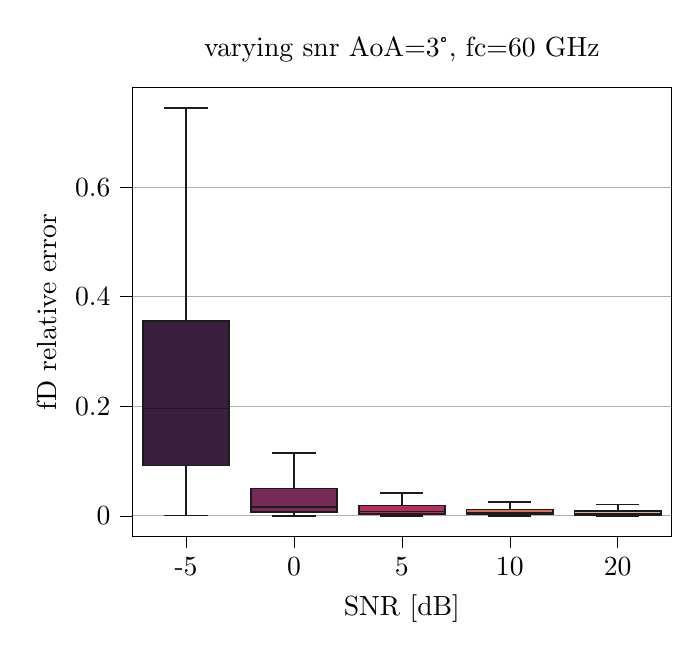
\begin{tikzpicture}

\definecolor{black28}{RGB}{28,28,28}
\definecolor{brown1814888}{RGB}{181,48,88}
\definecolor{burlywood231175145}{RGB}{231,175,145}
\definecolor{darkgray176}{RGB}{176,176,176}
\definecolor{darkslategray583162}{RGB}{58,31,62}
\definecolor{indianred21811088}{RGB}{218,110,88}
\definecolor{purple1194288}{RGB}{119,42,88}

\begin{axis}[
tick align=outside,
tick pos=left,
title={varying snr AoA=3°, fc=60 GHz},
x grid style={darkgray176},
xlabel={SNR [dB]},
xmin=-0.5, xmax=4.5,
xtick style={color=black},
xtick={0,1,2,3,4},
xticklabels={-5,0,5,10,20},
y grid style={darkgray176},
ylabel={fD relative error},
ymajorgrids,
ymin=-0.0372104854235092, ymax=0.781435519229455,
ytick style={color=black}
]
\path [draw=black28, fill=darkslategray583162, semithick]
(axis cs:-0.4,0.0918735177512096)
--(axis cs:0.4,0.0918735177512096)
--(axis cs:0.4,0.355175734311985)
--(axis cs:-0.4,0.355175734311985)
--(axis cs:-0.4,0.0918735177512096)
--cycle;
\path [draw=black28, fill=purple1194288, semithick]
(axis cs:0.6,0.00667261433766895)
--(axis cs:1.4,0.00667261433766895)
--(axis cs:1.4,0.0501069284459508)
--(axis cs:0.6,0.0501069284459508)
--(axis cs:0.6,0.00667261433766895)
--cycle;
\path [draw=black28, fill=brown1814888, semithick]
(axis cs:1.6,0.00360383774760779)
--(axis cs:2.4,0.00360383774760779)
--(axis cs:2.4,0.0188952405623862)
--(axis cs:1.6,0.0188952405623862)
--(axis cs:1.6,0.00360383774760779)
--cycle;
\path [draw=black28, fill=indianred21811088, semithick]
(axis cs:2.6,0.00231245028812295)
--(axis cs:3.4,0.00231245028812295)
--(axis cs:3.4,0.0116770094629587)
--(axis cs:2.6,0.0116770094629587)
--(axis cs:2.6,0.00231245028812295)
--cycle;
\path [draw=black28, fill=burlywood231175145, semithick]
(axis cs:3.6,0.00144293217840162)
--(axis cs:4.4,0.00144293217840162)
--(axis cs:4.4,0.00915934701075699)
--(axis cs:3.6,0.00915934701075699)
--(axis cs:3.6,0.00144293217840162)
--cycle;
\addplot [semithick, black28]
table {%
0 0.0918735177512096
0 0.00038618993159321
};
\addplot [semithick, black28]
table {%
0 0.355175734311985
0 0.744224337199774
};
\addplot [semithick, black28]
table {%
-0.2 0.00038618993159321
0.2 0.00038618993159321
};
\addplot [semithick, black28]
table {%
-0.2 0.744224337199774
0.2 0.744224337199774
};
\addplot [semithick, black28]
table {%
1 0.00667261433766895
1 1.45136945842529e-05
};
\addplot [semithick, black28]
table {%
1 0.0501069284459508
1 0.114649670068828
};
\addplot [semithick, black28]
table {%
0.8 1.45136945842529e-05
1.2 1.45136945842529e-05
};
\addplot [semithick, black28]
table {%
0.8 0.114649670068828
1.2 0.114649670068828
};
\addplot [semithick, black28]
table {%
2 0.00360383774760779
2 1.02239545421258e-05
};
\addplot [semithick, black28]
table {%
2 0.0188952405623862
2 0.0417178737555802
};
\addplot [semithick, black28]
table {%
1.8 1.02239545421258e-05
2.2 1.02239545421258e-05
};
\addplot [semithick, black28]
table {%
1.8 0.0417178737555802
2.2 0.0417178737555802
};
\addplot [semithick, black28]
table {%
3 0.00231245028812295
3 6.96606170944244e-07
};
\addplot [semithick, black28]
table {%
3 0.0116770094629587
3 0.0256934252546205
};
\addplot [semithick, black28]
table {%
2.8 6.96606170944244e-07
3.2 6.96606170944244e-07
};
\addplot [semithick, black28]
table {%
2.8 0.0256934252546205
3.2 0.0256934252546205
};
\addplot [semithick, black28]
table {%
4 0.00144293217840162
4 4.20312232222743e-06
};
\addplot [semithick, black28]
table {%
4 0.00915934701075699
4 0.0206606814446444
};
\addplot [semithick, black28]
table {%
3.8 4.20312232222743e-06
4.2 4.20312232222743e-06
};
\addplot [semithick, black28]
table {%
3.8 0.0206606814446444
4.2 0.0206606814446444
};
\addplot [semithick, black28]
table {%
-0.4 0.19600545232912
0.4 0.19600545232912
};
\addplot [semithick, black28]
table {%
0.6 0.0158563458368815
1.4 0.0158563458368815
};
\addplot [semithick, black28]
table {%
1.6 0.00789199157072155
2.4 0.00789199157072155
};
\addplot [semithick, black28]
table {%
2.6 0.00498254904229145
3.4 0.00498254904229145
};
\addplot [semithick, black28]
table {%
3.6 0.00359930103696884
4.4 0.00359930103696884
};
\end{axis}

\end{tikzpicture}
